\documentclass[tikz,border=8pt]{standalone}
% Shared look for every TikZ diagram. Load with \input{../../tools/tikz-style.tex}
\usepackage[T1]{fontenc}
\usepackage{lmodern}
\renewcommand{\sfdefault}{lmr}  % diagrams use the same serif as the text
\usetikzlibrary{arrows.meta, positioning, shapes.geometric, calc, fit, backgrounds}
\definecolor{cblue}{HTML}{4C78A8}
\definecolor{corange}{HTML}{F58518}
\definecolor{cgreen}{HTML}{54A24B}
\definecolor{cred}{HTML}{E45756}
\definecolor{cpurple}{HTML}{B279A2}
\definecolor{cgrey}{HTML}{6B6B6B}
\tikzset{
  every picture/.style={font=\sffamily, line width=1.2pt},
  box/.style={draw=#1, fill=#1!12, rounded corners=4pt, align=center, inner sep=7pt, minimum height=1.1cm},
  box/.default=cgrey,
  arrow/.style={-{Stealth[length=3mm]}, draw=cgrey, line width=1.4pt},
  title/.style={font=\sffamily\bfseries\Large},
  note/.style={font=\sffamily\small, text=cgrey, align=center},
}
\AtBeginDocument{\hyphenpenalty=10000 \exhyphenpenalty=10000}

\begin{document}
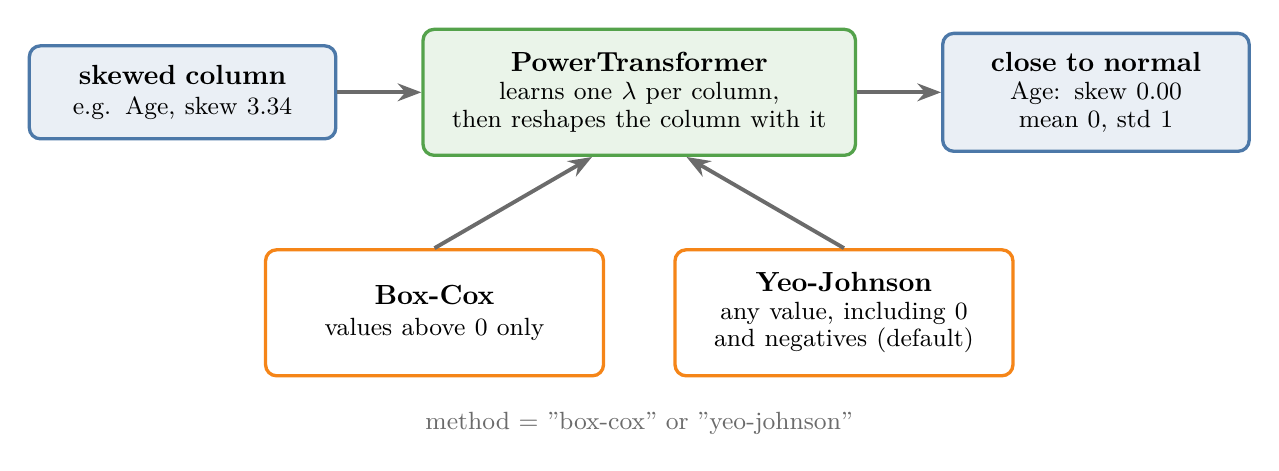
\begin{tikzpicture}
  \node[box=cblue, text width=3.4cm] (in) at (0,0) {\textbf{skewed column}\\[-1pt]\small e.g. Age, skew 3.34};
  \node[box=cgreen, text width=5cm, minimum height=1.6cm] (pt) at (5.8,0)
    {\textbf{PowerTransformer}\\[-1pt]\small learns one $\lambda$ per column,\\[-2pt]\small then reshapes the column with it};
  \node[box=cblue, text width=3.4cm] (out) at (11.6,0) {\textbf{close to normal}\\[-1pt]\small Age: skew 0.00\\[-2pt]\small mean 0, std 1};
  \draw[arrow] (in) -- (pt);
  \draw[arrow] (pt) -- (out);
  \node[box=corange, fill=white, text width=3.8cm, minimum height=1.6cm] (bc) at (3.2,-2.8)
    {\textbf{Box-Cox}\\[-1pt]\small values above 0 only};
  \node[box=corange, fill=white, text width=3.8cm, minimum height=1.6cm] (yj) at (8.4,-2.8)
    {\textbf{Yeo-Johnson}\\[-1pt]\small any value, including 0\\[-2pt]\small and negatives (default)};
  \draw[arrow] (bc.north) -- ($(pt.south)+(-0.6,0)$);
  \draw[arrow] (yj.north) -- ($(pt.south)+(0.6,0)$);
  \node[note] at (5.8,-4.2) {method = "box-cox" or "yeo-johnson"};
\end{tikzpicture}
\end{document}
